\section{Theorie}
\label{sec:Theorie}

Im Folgenden wird Grundprinzip von Operationsverstärken erklärt, sowie die möglichen Funktionen in Kombination mit 
weiteren elektrischen Bauteilen beschrieben.

\subsection{Operationsverstärker}

\subsubsection{Idealer und realer OP-Amp}
Operationsverstärker (OP-Amps) sind elektrische Bauteile, die die Differenz von zwei eingehenden Signalen verstärken können.
In \autoref{fig:opamps} sind eine Ausführung eines LM741-OP-Amps sowie der prinzipielle Aufbau mit Pin-Konfiguration dargestellt.

\begin{figure}[H]
    \centering
    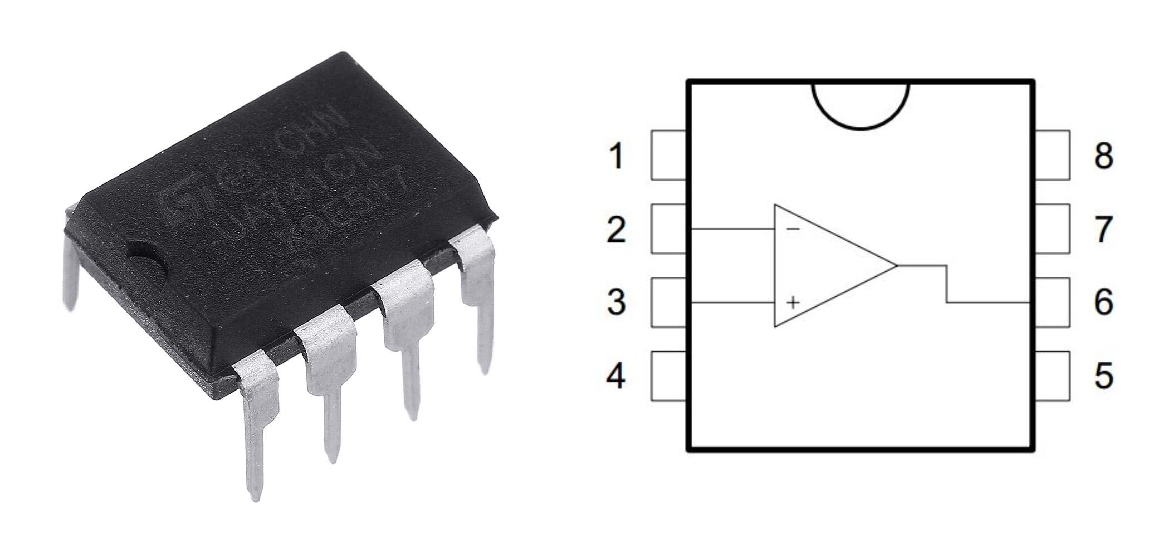
\includegraphics[width=\textwidth]{../theorie_bilder/opamp.png}
    \caption{Links: LM741. Die Auskerbung gibt die Orientierung des Verstärkers an. Rechts: Pin-Konfiguration eines LM741 in einem DIL8 Housing.}
    \label{fig:opamps}
\end{figure}

Pin 1 und 5 werden als Offset-Null 1 und 2 bezeichnet. Pin 2 ist der sogenannte Inverting Input, Pin 3 der Non-Inverting Input. Pin 4 ist für die negative Betriebsspannung, Pin 7 für die positive Betriebsspannung. Pin 6 ist der Output, Pin 8 hat keinen Nutzen.

Der Output $A_\text{o}$ durch den Inverting Input mit Amplitude $A_-$ und dem Non-Inverting Input mit Amplitude $A_+$ wird beschrieben durch

\begin{equation*}
    A_\text{o} = A \cdot (A_+ - A_-),
\end{equation*}

dabei ist $A$ die Amplification. In einem idealen OP-Amp ist dieser unendlich hoch, was jede noch so kleine Signaldifferenz verstärken würde. In der Realität ist dies nicht möglich, 
weshalb dieser nur sehr hoch eingestellt wird. Die Betriebsspannungen bestimmen die Range des Outputs, weshalb diese so gewählt werden, dass sie symmetrisch um $\SI{0}{\volt}$ liegen.

Des Weiteren unterscheiden sich ideale und reelle OP-Amps durch insbesondere ihre Impedanzen. Input-Impedanzen sind idealerweise unendlich hoch, sodass es einen Strom-Rückfluss gibt,
während sie in Realität nur endlich hoch eingestellt werden können. Die Output-Impedanzen sind idealerweise 0, realistisch sind aber nur sehr kleine, von Null verschiedene Werte.
Die Bandbreite der ausgebbaren Frequenzen ist im idealen OP-Amp unendlich, im reellen aber endlich. Die Slew-Rate, also die Verzögerung zwischen Input und Output, ist im perfekten OP-Amp null, aber in Realität im Bereich von wenigen $\si{\volt\per\micro\second}$.

Der Output eines OP-Amps kann als Feedback für den Input verwendet werden. Wird er in den Inverting Input gespeist,
spricht man von negativem Feedback. Negatives Feedback stabilisiert den Output und erhöht die Bandbreite. Positives Feedback, wenn der Output in den Non-Inverting Input gespeist wird,
saturiert den Output und ermöglicht Oszillationen, insbesondere kann somit ein Schmitt-Trigger gebaut werden.

Über Feedback-Schaltungen mit verschiedenen elektrischen Komponenten können weitere Operatoren realisiert werden.

\subsubsection{Inverting-Amplifier}

Der Aufbau eines Inverting-Amplifiers ist in \autoref{fig:inv_ampl} dargestellt.

\begin{figure}[H]
    \centering
    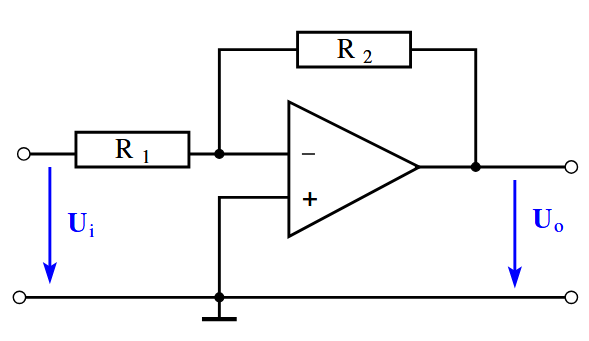
\includegraphics[width=\textwidth]{../theorie_bilder/inv_ampl.png}
    \caption{Aufbaue eines Inverting-Amplifiers mit zwei Widerständen und einem OP-Amp.}
    \label{fig:inv_ampl}
\end{figure}


